Como parte de nuestra estrategia de aprendizaje no supervisado, se implementó un modelo de autoencoder con el objetivo de predecir y comprender el comportamiento del usuario utilizando un conjunto de datos complejo. El autoencoder, una herramienta avanzada en el campo del aprendizaje automático, se especializa en identificar patrones y características intrínsecas dentro de grandes volúmenes de datos. Esta implementación fue clave para descifrar las complejidades y matices del comportamiento del usuario, permitiendo al modelo aprender de manera autónoma sin la necesidad de etiquetas predefinidas. La aplicación de este modelo de autoencoder facilitó el análisis detallado de los datos, contribuyendo significativamente a la comprensión de patrones subyacentes y tendencias de comportamiento de los usuarios.

\subsection{Preprocesamiento y Preparación de Datos}
El proceso de preparación de los datos para el entrenamiento del modelo comenzó con la carga del conjunto de datos desde un archivo CSV. Esta etapa inicial fue seguida por una meticulosa fase de limpieza de datos, un paso crucial para asegurar la calidad y la fiabilidad de los datos que se utilizarían en el entrenamiento del modelo. Las operaciones de preprocesamiento realizadas en los datos incluyeron las siguientes:

\begin{itemize}
    \item \textbf{Normalización de Fechas:} En el proceso de preparación de los datos, la columna \textquotedblleft fecha\_evento\textquotedblright, que contenía información relevante de fecha y hora, fue objeto de una cuidadosa división y estandarización. Este procedimiento se realizó con el fin de asegurar que los datos temporales se presentaran en un formato uniforme y coherente, facilitando su utilización y análisis posterior. La estandarización de esta columna es un paso crítico, ya que permite que las marcas temporales sean procesadas de manera efectiva por el modelo, y garantiza la consistencia en la interpretación de los datos temporales a lo largo de todo el conjunto de datos. La adecuada preparación y formato de los datos temporales son esenciales para cualquier análisis que involucre aspectos temporales y secuenciales.
    \item \textbf{Eliminación de columnas innecesarias:} Tras el proceso de codificación, las columnas originales de \textquotedblleft método\textquotedblright y \textquotedblleft canal\textquotedblright en nuestro conjunto de datos fueron eliminadas. Esta decisión se tomó para mantener el dataset conciso y enfocado exclusivamente en las características más relevantes para el análisis y el modelado. La eliminación de estas columnas originales, después de haber sido transformadas en un formato más adecuado para el procesamiento por el modelo, es una práctica estándar en el preprocesamiento de datos. Este enfoque ayuda a reducir la dimensionalidad del conjunto de datos y asegura que el modelo se centre en los atributos que aportan información valiosa y significativa, evitando así la redundancia y el ruido innecesario.
    \item \textbf{Transformación Temporal Adicional:} Se implementaron codificaciones one-hot en las columnas \textquotedblleft fecha\textquotedblright, \textquotedblleft hora\textquotedblright y \textquotedblleft día de la semana\textquotedblright de nuestro conjunto de datos. Este enfoque de codificación fue elegido para mejorar la representación de los aspectos temporales en el análisis de los datos.
\end{itemize}

\subsection{Codificación One-Hot}
En relación con las variables categóricas \textquotedblleft método\textquotedblright y \textquotedblleft canal\textquotedblright, se aplicó la técnica de codificación One-Hot para su adecuada transformación. Esta técnica es un componente esencial en la preparación de datos categóricos para su incorporación en modelos de aprendizaje automático. Consiste en convertir estas variables en un formato numérico, optimizando así su interpretación y manejo por el modelo. Con la codificación One-Hot, cada categoría única de estas variables se traduce en una columna independiente en el conjunto de datos. En estas columnas recién creadas, la presencia de una categoría específica en una instancia se denota con un "1", mientras que su ausencia se representa con un "0". Este método facilita que el modelo reconozca y procese las características categóricas de manera eficiente, sin presuponer un orden jerárquico entre ellas, lo cual es vital para lograr un análisis preciso y una modelización efectiva.


\begin{figure}[H]
    \begin{minipage}[t]{0.9\textwidth}
        \caption{Preparación y codificación one-hot de los datos}
        \label{codificación_autoencoder}        
    \end{minipage}

    \vspace{10pt}

    \begin{minipage}[b]{0.9\textwidth}
        \centering
        \includegraphics[width=\textwidth]{img/codificación one-hhot.jpg}        
    \end{minipage}

    \begin{minipage}[t]{0.9\textwidth}
        Fuente: Elaboración propia.
    \end{minipage}
\end{figure}


\subsection{Construcción y Entrenamiento del Modelo}

El dataset fue dividido en conjuntos de entrenamiento y validación. Luego, se construyó la arquitectura del autoencoder con capas densas y normalización por lotes, utilizando una función de activación \textquotedblleft tanh\textquotedblright para las capas codificadoras y \textquotedblleft relu\textquotedblright para las decodificadoras. Se implementó un mecanismo de EarlyStopping para prevenir el sobreentrenamiento y mejorar la generalización del modelo.

Un autoencoder es un tipo de red neuronal utilizada en el aprendizaje no supervisado, que tiene como objetivo aprender una representación (codificación) de un conjunto de datos, típicamente para reducción de dimensionalidad, aprendizaje de características, o descompresión de datos. La particularidad de los autoencoders reside en que están diseñados para reconstruir su entrada en la salida, pasando la información a través de una serie de capas que primero comprimen los datos (codificador) y luego los reconstruyen (decodificador).

En el caso de un autoencoder con \textquotedblleft capas densas" (también conocidas como \textquotedblleft capas completamente conectadas"), cada neurona en una capa está conectada a todas las neuronas en la capa siguiente. Este tipo de arquitectura es una de las más comunes en las redes neuronales y es particularmente útil para aprender patrones complejos y no lineales en los datos.

\subsubsection{Construcción del Codificador}
En la parte del codificador, los datos de entrada pasan a través de capas densas, donde se reduce gradualmente la dimensionalidad. Este proceso se logra reduciendo el número de neuronas en capas sucesivas, obligando así a la red a aprender una representación comprimida de los datos de entrada. Las funciones de activación como \textquotedblleft tanh" (tangente hiperbólica) pueden ser usadas aquí para introducir no linealidades en el modelo, permitiendo que el codificador aprenda representaciones más complejas.

\subsubsection{Construcción del Decodificador} 
La segunda parte del autoencoder es el decodificador, donde la representación comprimida se procesa a través de otras capas densas para reconstruir los datos de entrada. El objetivo es que la salida sea lo más cercana posible a la entrada original. Las funciones de activación como \textquotedblleft relu" (Rectified Linear Unit) son comunes en esta etapa, proporcionando una manera eficiente y efectiva de realizar operaciones no lineales.

\begin{figure}[H]
    \begin{minipage}[t]{0.9\textwidth}
        \caption{Arquitectura del modelo autoencoder}
        \label{arquitectura_autoencoder}        
    \end{minipage}

    \vspace{10pt}

    \begin{minipage}[b]{0.99\textwidth}
        \centering
        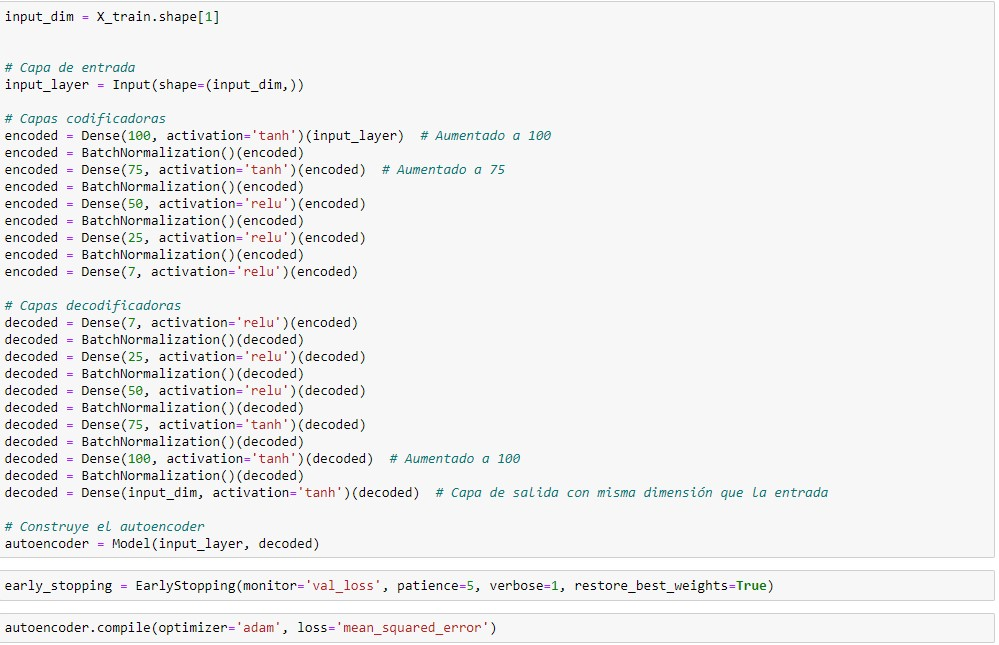
\includegraphics[width=\textwidth]{img/Arquitectura modelo autoencoder.jpg}        
    \end{minipage}

    \begin{minipage}[t]{0.9\textwidth}
        Fuente: Elaboración propia.
    \end{minipage}
\end{figure}

El entrenamiento del autoencoder se realizó adoptando un enfoque iterativo y dinámico, donde uno de los aspectos clave fue el monitoreo de la pérdida de validación a lo largo de las iteraciones del entrenamiento, conocidas como "épocas". En el contexto del aprendizaje automático y especialmente en el entrenamiento de redes neuronales, una "época" se refiere a un ciclo completo de pase de todos los datos de entrenamiento a través del modelo.

Una época representa una iteración completa sobre el conjunto de datos de entrenamiento. Durante una época, el modelo procesa cada muestra del conjunto de entrenamiento una vez, permitiendo que el modelo aprenda de los datos. Esto implica que si tenemos un conjunto de datos de entrenamiento con, por ejemplo, 1000 muestras y el modelo se entrena durante 10 épocas, entonces cada muestra habrá sido utilizada 10 veces para ajustar los parámetros del modelo.

Las épocas son fundamentales en el proceso de entrenamiento de un modelo de aprendizaje automático:

\subsubsection{Aprendizaje Progresivo} 
Con cada época, el modelo tiene la oportunidad de aprender y adaptarse a los datos, ajustando sus parámetros (como los pesos en una red neuronal) para minimizar el error o la pérdida.

\subsubsection{Evaluación y Ajustes} 
Al monitorear la pérdida, especialmente la pérdida de validación, al final de cada época, se puede evaluar cómo está aprendiendo el modelo. Si la pérdida de validación deja de mejorar o comienza a aumentar, puede ser una señal de sobreajuste, indicando que el modelo está aprendiendo a memorizar los datos de entrenamiento en lugar de generalizar a partir de ellos.

\subsubsection{Término del Entrenamiento} 
El número de épocas también juega un papel crucial en la determinación de cuándo detener el entrenamiento. Demasiadas épocas pueden llevar a sobreajuste, mientras que muy pocas pueden resultar en un modelo subajustado.

\begin{figure}[H]
    \begin{minipage}[t]{0.9\textwidth}
        \caption{Entrenamiento del modelo autoencoder}
        \label{entrenamiento_autoencoder}        
    \end{minipage}

    \vspace{10pt}

    \begin{minipage}[b]{0.99\textwidth}
        \centering
        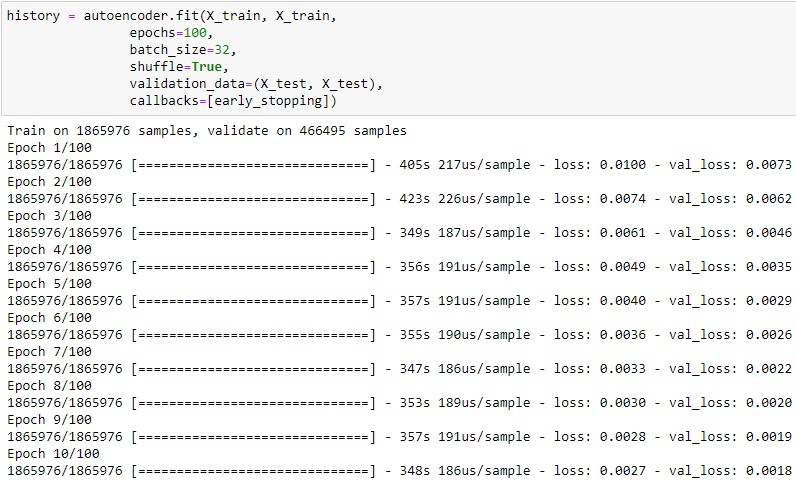
\includegraphics[width=\textwidth]{img/Entrenamiento autoencoder.jpg}        
    \end{minipage}

    \begin{minipage}[t]{0.9\textwidth}
        Fuente: Elaboración propia.
    \end{minipage}
\end{figure}

\subsection{Resultados y Evaluación}

El modelo final demostró una sólida capacidad de reconstrucción y no mostró signos de sobreajuste, como se evidencia en los gráficos de pérdida de entrenamiento. Este autoencoder está ahora listo para ser utilizado para transformar los datos en una representación de menor dimensión, lo cual facilitará la aplicación de técnicas de clustering para la segmentación de usuarios y la detección de patrones de comportamiento anómalos.

\begin{figure}[H]
    \begin{minipage}[t]{0.9\textwidth}
        \caption{Gráfico del entrenamiento del modelo autoencoder}
        \label{gráfico_autoencoder}        
    \end{minipage}

    \vspace{10pt}

    \begin{minipage}[b]{0.9\textwidth}
        \centering
        \includegraphics[width=\textwidth]{img/Gráfico entrenamiento autoencoder.png}        
    \end{minipage}

    \begin{minipage}[t]{0.9\textwidth}
        Fuente: Elaboración propia.
    \end{minipage}
\end{figure}

\subsection{Conclusión del Modelo de Autoencoder}

El autoencoder se diseñó para transformar datos de alta dimensión en una representación de menor dimensionalidad, lo cual es un paso fundamental en el pre-procesamiento para algoritmos de clustering.

Sin embargo, el propósito inicial del autoencoder no era predecir comportamientos futuros o tendencias, sino más bien identificar patrones intrínsecos y datos atípicos dentro del conjunto de datos existente. Dado que el objetivo central del proyecto es la predicción del comportamiento, se ha determinado que el autoencoder no cumple con los requisitos necesarios para avanzar hacia este nuevo objetivo.

Por tanto, hemos decidido no continuar con el desarrollo e implementación de este modelo en su forma actual. En cambio, nos enfocaremos en la búsqueda y aplicación de modelos predictivos más adecuados que estén alineados con las metas de pronosticar el comportamiento futuro y que puedan ofrecer insights más directos para la toma de decisiones y estrategias proactivas.

Este cambio de dirección subraya la importancia de una alineación clara entre las herramientas de modelado seleccionadas y los objetivos específicos del proyecto. Aunque el autoencoder es una herramienta poderosa para ciertas aplicaciones, en este caso, se ha reconocido que no es la solución óptima para las necesidades proyectadas.

Sin embargo, es importante destacar que el autoencoder es una herramienta extremadamente útil para identificar anomalías en patrones de comportamiento.
